\documentclass[spanish, fleqn]{article}
\usepackage{babel}
\usepackage[utf8]{inputenc}
\usepackage{fourier}
\usepackage{icomma}
\usepackage{amsmath, amsfonts, amsthm, fourier, amssymb}
\usepackage[colorlinks, urlcolor=blue]{hyperref}
\usepackage{graphicx}
\usepackage{listings}

\usepackage{graphicx}
\graphicspath{ {plt/} }

\newcommand{\num}{1}
\title{Tarea \num\\
       \large Algoritmos y Complejidad\\[3ex]
       \emph{``Tonteando\ldots''}}
\author{Sebastián Bórquez González\\201573015-6}
\date{2 de Abril, 2018}

\begin{document}

\maketitle

	El enunciado nos entrega una función $f$ sobre $x$ tal que se cumple:
	\begin{align*}
	y &= f(x)\\
	x &= f^{-1} (y)
	\end{align*}
	
	Pero solo se conoce a $f$ en puntos discretos los cuales son entregados en una tabla.
	
	Además se trabaja bajo el supuesto de que existe $f^{-1}$ por lo que se debe cumplir que $f$ sea \textbf{biyectiva}.	
		
  \begin{enumerate}
  \item % 20181t1p1
  Dado una lista puntos $(x,y)$ se debe crear una función para poder interpolar utilizando estos puntos el valor de $y$ para un nuevo valor de $x$. 
  
  Se decide implementar de manera implícita. Se compararán dos métodos implicitos: \textbf{Lagrange} y \textbf{Newton}.
  
  Para Lagrange, dado a la complejidad $O(n^2)$ de la forma original se implementará \textbf{Lagrange Baricentrico}, el cual es recomendable dado que es númericamente estable.
  
Esta forma pide calcular: 

	$$p(x) = \frac{\sum_{0\leq j\leq n}\frac{w_i f(x_i)}{x-x_j}}{\sum_{0\leq j\leq n}{\frac{w_i}{x-x_j}}}$$  
   
    $$w_i = \left( \prod_{0\leq k\leq n}[k \neq j] (x_j - x_k) \right)^{-1}$$
    
    Esta forma nos entrega una versión fácil de vectorizar, debido a terminos frecuentes y a operaciones que se realizan dentro de iteraciones (sumatoría y multiplicatoria).
    
    Para Newton, se utiliza \textbf{Diferencias divididas}, el algoritmo se separa en dos partes: Calcular los coeficientes $A_i$ del polinomio utilizando las diferencias divididas. Luego armar el polinomio usando:
    
    $$p(x)=\sum_{0\leq i\leq n-1}\left( A_i \prod_{0\leq j \leq i-2}(x - x_j)\right)$$
    
    Como resultados obtenemos:
    
   \begin{figure}[h]
    \caption{Interpolación de los puntos}
    \centering 
 	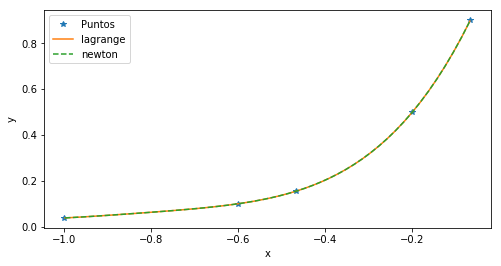
\includegraphics[scale=0.6]{interpolacion1.png}
   \end{figure}
  
	Como se puede observar, ambos métodos generan al mismo polinomio.
	
	Pero, ¿Cuál método elegir?
	Se realizaron unas pruebas de velocidad y error para dos cantidades de puntos de una función $f(x) = cos(x) + 2 sin(x) + 0.5x$.
	
	Se utilizan dos 5 y 50 puntos equiespaciados en $[-2\pi, 2\pi]$. Luego se calcula el error en todo el rango $[-2\pi, 2\pi]$.
		\begin{center}
	\begin{tabular}{|l|c|c|l|}
	\hline
	Puntos & Lagrange T$[\mu s]$& Newton T$[\mu s]$& $\frac{\text{Error}_{Lagrange}}{\text{Error}_{Newton}}$\\
	\hline
	5	& 49.7 & 9.38 & $\thickapprox$ 1\\
	\hline
	50 & 353 & 518 & $\thickapprox$ 100\\
	\hline
	\end{tabular}
	

	\small{\textit{Tiempo calculado usando '\%timeit'}}
	\end{center}
  
  
  Como conclusión, podemos observar que para pocos puntos, mi implementación del método de Newton es más rápido, aunque ambos tienen el mismo error. En el caso de darnos más puntos, mi implementación de Lagrange es más rápida, pero tiene un mayor error.
  
  Dado el caso particular de este problema, al ser solo 5 puntos, se decide usar la implementación de \textbf{diferencias divididas}.
  
  \item % 20181t1p2
  Se nos pide implementar el método de la secante, lo cual se hace de manera bastante directa. Partiendo con $x_0$ , $x_1$ se calculan valores sucesivos usando:
  
  $$x_{n+2} = x_{n+1} - f(x_{n+1}) \cdot \frac{x_{n+1}-x_{n}}{f(x_{n+1}) - f(x_n)}$$ 
  
  Se ha de suponer que para los $x$ dados, el termino $f(x_{n+1}) - f(x_n)$ nunca indefinirá a la división.
  
  El algoritmo realizará la iteración hasta que  
  el $f(x_{n+2})$ esté a lo más a una distancia de $\epsilon$ (tolerancia) del 0, o si el algoritmo a iterado una cierta cantidad de veces (prevención a que no converja).
  
  \item % 20181t1p3
	Se desea obtener el valor de $x^*$ para la evaluación de la función $f^{-1} (y^*)$ con $y^*=0.3$. 
	
	Escrito en terminos de $f$, buscamos un $x^*$ que satisfaga la ecuación: $f(x^*) = y^*$, o lo que es lo mismo, buscar el $x$ de la intercepción de las funciones $y = f(x)$ e $ y = y^*$.
	  
     \begin{figure}[h]
     \caption{Intercepción entre $y=f(x)$ e $y=y^*$}
    \centering 
 	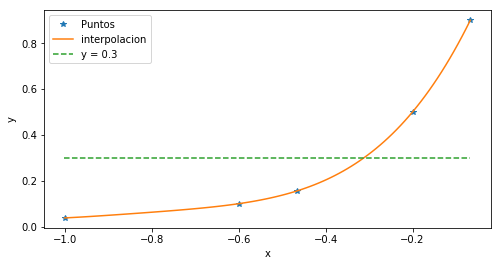
\includegraphics[scale=0.6]{intercepcion.png}
   \end{figure}
	
	Partiendo de esta idea, la intercepción es $f(x) = y^*$. Buscar el punto de intercepción es equivalente a buscar el $x^*$ que cumpla $g(x) = 0$, con $g$ definida como $g(x) = f(x) - y^*$.
	
	De esta forma, podemos utilizar el método de la secante para encontrar un cero de $g$, con la diferencia de que esta vez no se utiliza un $f$ en concreto, sino que la interpolación.
  
	Para la elección de los puntos iniciales se tomó en cuenta los valores de la tabla, y confirmados por la interpolación, los puntos presentan un comportamiento creciente, por lo que se determinó que $0.3$ debería encontrarse entre $x_0 = -0.467$ y $x_1=-0.2$.
	
  
	Finalmente, el resultado de nuestro calculo resultó:
	
		$$x^* = -0.31190496815431695$$  
  
  \item % 20181t1p4
  
  Una forma diferente de aproximarse al problema es interpolando la función inversea $f^{-1}$. Para esto utilizamos el mismo método de interpolación con la salvedad de que la lista de puntos $X$ e $Y$ están invertidos y se evalua al polinomio con el valor de $y^*$, para este caso en particular, $y^* = 0.3$.
  
  Este método aparenta ser una forma correcta y directa para obtener el valor $x^*$. Sin embargo, como resultado obtenemos un valor diferente al calculado en la respuesta anterior.
  
  $$x^* = -0.50864947547118666$$
  
   \begin{figure}[h]
	\caption{Polinomio de interpolación de $f^{-1}$}   
	\centering
 	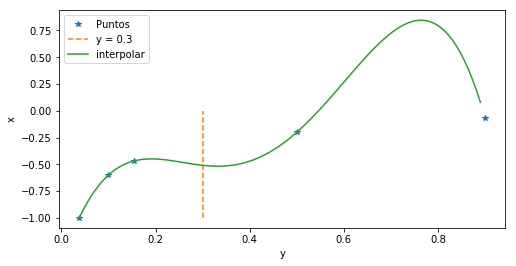
\includegraphics[scale=0.6]{interpolacioninversa.png}
   \end{figure}
  
  
  ¿Cuál es la razón de que  se hayan obtenido resultados diferentes?
  
   La causa la podemos encontrar al revisar más detalladamente la interpolación. Se puede observar en la forma del polinomio de interpolación.
     
  Como se puede apreciar, partimos de la idea de que existía $f^{-1}$, por lo que $f$ debe ser biyectiva, por consecuencia $f^{-1}$ debe ser biyectiva. En esta interpolación se puede apreciar de que esto último no se cumple para el polinomio interpolador, por lo que utilizar este método para aproximar valores de la función inversa puede no entregarnos un resultado correcto, lo que explica la aproximación erronea.
  
   En conclusión, interpolar la función inversa de algún $f$ no necesariamente nos entrega la inversa del polinomio de interpolación de este $f$.
  \end{enumerate}

\end{document}


